                                                                                                                                                                                                                                                                                                                                                                                                                                                                                                                                                                                                                                                                                                                                                                                                                                                                                                                                                                                                                                                                                                                                                                                                                                                                                                                                                                                                      \begin{frame}
\titlepage
\end{frame}
\begin{frame}
\frametitle{Problem Statement-Triangle Exercise}


\begin{enumerate}[label=(\roman*)]
\item ABC and DBC are two triangles on the same
base BC. If AD intersects BC at O, show that\\
$\frac{ar(ABC)}{ar(DBC)}=\frac{AO}{DO}$\\
\end{enumerate}
\textbf{Soln:}\\
\begin{figure}
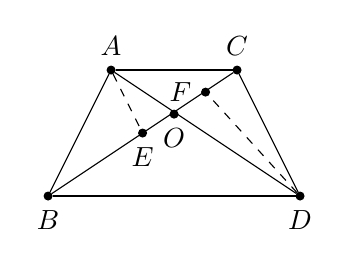
\begin{tikzpicture}
[scale = 0.4,>=stealth,point/.style = {draw, circle, fill = black, inner sep = 1pt},]
\node (A) at (2,4)[point,label=above :$A$] {};
\node (B) at (0,0)[point,label=below :$B$] {};
\node (C) at (6,4)[point,label=above :$C$] {};
\node (D) at (8,0)[point,label=below :$D$] {};
\node (E) at (3,2)[point,label=below :$E$] {};
\node (F) at (5,3.3)[point,label=left :$F$] {};
\node (O) at (4,2.6)[point,label=below :$O$] {};
\draw (D)--(A);
\draw (A)--(B);
\draw (B)--(C);
\draw (A)--(C);
\draw (B)--(D);
\draw (C)--(D);
\draw [dashed] (A) -- (E);
\draw [dashed] (D) -- (F);
\tkzMarkRightAngle[draw=red,size=.4](A,E,C)
\tkzMarkRightAngle[draw=red,size=.4](D,F,E)
\end{tikzpicture}
\includegraphics[scale=0.2]{./figs/priyanka.png}
\end{figure}
\end{frame}
\begin{frame}
\begin{align*}
AE\perp BC , DF\perp BC\\
Area of \triangle{ABC} = \frac{1}{2}BC*AE\\
Area of \triangle{DBC} = \frac{1}{2}BC*DF\\
\frac{ar\triangle{ABC}}{ar\triangle{DBC}}=\frac{\frac{1}{2}BC*AE}{\frac{1}{2}BC*DF}\\  
\frac{ar\triangle{ABC}}{ar\triangle{DBC}}=\frac{AE}{DF}\\
\frac{AE}{DF}=\frac{AO}{DO}\\
\angle{AEO}=\angle{DFO}..... RA\\
\angle{AEO}=\angle{DOF}..... VOA\\
\triangle{AOE} \sim \triangle{DOF}\\
\frac{AE}{DF}=\frac{AO}{DO}\\
\end{align*}

\end{frame}